% 第5章第2节：基、维数与坐标（线性无关与张成、基、维数、坐标与坐标变换）。

\section{基、维数与坐标}
\label{sec:ls-bases-dimension-coordinates}

上一节规定了在什么范围里作线性组合，但还没有回答怎样用有限个数记录一个对象。思路是选定一组方向，把对象写成它们的线性组合，用组合系数代替对象。

这要求依次回答几个问题：一组方向能到达哪些对象；到达同一个对象的系数是否唯一；怎样挑出一组既够用又不重复的方向作为“尺子”；不同的尺子是否总含同样多根，即空间有多大；选定尺子以后，系数怎样代替对象参与计算，换一把尺子系数怎样换算。前一个问题的答案是后一个问题的前提，所以按这个顺序展开。

\subsection{张成与线性无关}

\paragraph{张成}
\phantomsection
\label{sec:ls-span}
在平面上，两个不共线方向的加权组合能取到每一个点；只有一个方向时，无论怎样加权，结果都停在过原点的一条直线上。要描述一组方向“能到达哪里”，先给它们的全部线性组合命名：给定$\bm v_1,\ldots,\bm v_k\in V$，集合
\begin{equation}
 \operatorname{span}\{\bm v_1,\ldots,\bm v_k\}
 =\left\{\sum_{j=1}^k a_j\bm v_j:a_j\in\mathbb R\right\}
 \label{eq:ls-span}
\end{equation}
称为这组向量的\term{张成空间}（span）。

两个线性组合再作线性组合，仍是这组向量的线性组合，所以张成空间对线性组合封闭，是$V$的子空间。

任何包含$\bm v_1,\ldots,\bm v_k$的子空间都必须含有它们的全部线性组合，所以张成空间是包含这组向量的最小子空间。若$\operatorname{span}\{\bm v_1,\ldots,\bm v_k\}=V$，就说这组向量张成$V$，也称它们是$V$的一个生成组。

在$\mathbb R^m$中，把$\bm v_1,\ldots,\bm v_k$排成矩阵$\bm V$的各列，按列读法$\sum_ja_j\bm v_j=\bm V\bm a$，所以张成空间就是$\bm V$乘上全部系数向量所得的输出集合$\{\bm V\bm a:\bm a\in\mathbb R^k\}$，第~\ref{sec:ls-kernel-image}节将把它称为$\bm V$的列空间。如图~\ref{fig:ls-linear-combination-span}所示，两个不共线方向的组合取遍整个平面，单个方向的组合只是一条直线。
\begin{figure*}[htbp]
  \centering
  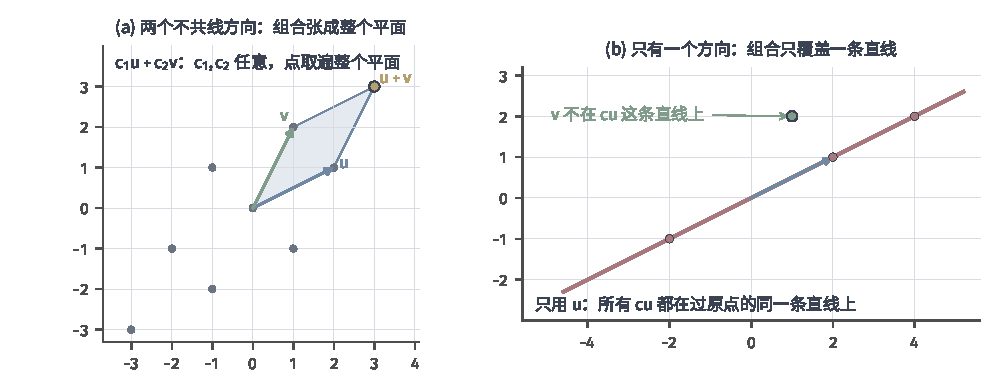
\includegraphics[width=169mm]{figures/00-shared/mathematical-preliminaries-upper/02-linear-spaces/matplotlib/ls-linear-combination-span/ls-linear-combination-span.pdf}
  \caption{两个方向与一个方向的张成范围。左：$\bm u=(2,1)$（蓝箭头）与$\bm v=(1,2)$（绿箭头）的全部加权组合取遍整个平面，浅蓝平行四边形标出$0,\bm u,\bm u+\bm v,\bm v$，灰点为整数系数格点，黄点为$\bm u+\bm v=(3,3)$。右：只有$\bm u$一个方向时，组合$\{c\bm u\}$只是过原点的一条直线（红线），$\bm v$不在其上。两图坐标等比例，为解析教学例。}
  \label{fig:ls-linear-combination-span}
\end{figure*}

\paragraph{线性无关}
\phantomsection
\label{sec:ls-linear-dependence}
张成告诉我们哪些对象能被表示，却没有说明表示方式是否只有一种。若同一个对象可以用两组不同的系数写出，某些方向就是多余的。两组系数相减，就得到零向量的一个系数不全为零的表示，所以判断冗余，只需看零向量能否被非平凡地表示。若
\begin{equation}
 a_1\bm v_1+\cdots+a_k\bm v_k=\bm0
 \label{eq:linear-algebra-independence-relation}
\end{equation}
仅在全部$a_j=0$时成立，就称这组向量\term{线性无关}（linearly independent）；否则称为\term{线性相关}（linearly dependent），即存在不全为零的系数使式\eqref{eq:linear-algebra-independence-relation}成立。线性相关时挑出一个非零系数$a_j$并移项，就能把$\bm v_j$写成其余向量的线性组合，说明这个方向重复了已有方向能到达的范围。在$\mathbb R^m$中，线性无关就是齐次方程$\bm V\bm a=\bm0$只有零解；第~\ref{sec:ls-gram-orthogonality}节还将说明，它等价于Gram矩阵$\bm V^\top\bm V$正定。

贯穿例的两列几乎同向，它们是否线性无关？
\begin{example}[近共线的两列仍线性无关]
\label{ex:ls-nearly-collinear-independence}
给定：式~\eqref{eq:linear-algebra-nearly-collinear-design}中的$\bm c_1=(1,1,1)^\top$、$\bm q=(0,1,-1)^\top$与$\bm c_2=\bm c_1+\varepsilon\bm q$。

验证：先看$\bm c_1$与$\bm q$。$\alpha\bm c_1+\beta\bm q=(\alpha,\ \alpha+\beta,\ \alpha-\beta)^\top$为零时，第一坐标给出$\alpha=0$，第二坐标再给出$\beta=0$，所以$\bm c_1,\bm q$线性无关。再看两列：
\[
 a_1\bm c_1+a_2\bm c_2=(a_1+a_2)\bm c_1+a_2\varepsilon\bm q .
\]
它为零时，由$\bm c_1,\bm q$线性无关得$a_1+a_2=0$与$a_2\varepsilon=0$。

结论：$\varepsilon\neq0$时只能$a_2=0$，进而$a_1=0$，两列线性无关；$\varepsilon=0$时$\bm c_1-\bm c_2=\bm0$，两列线性相关。
\end{example}
所以“两列几乎同向”和线性无关是两回事。线性无关是精确的是非判断，只要$\varepsilon\neq0$就成立；几乎同向描述的是接近退化的程度，要由夹角或Gram矩阵衡量，第~\ref{sec:ls-inner-product-definition}节把这种情形称为近共线。

\paragraph{表示的存在与唯一}
“能表示哪些对象”和“表示是否冗余”是两个独立的问题，分别由张成与线性无关回答。下面的例子在平面上把二者分开。
\begin{example}[足够、不够与冗余的方向组]
\label{ex:ls-redundant-spanning-set}
给定：$\mathbb R^2$中的$\bm v_1=(1,0)^{\top}$、$\bm v_2=(0,1)^{\top}$与$\bm v_3=(1,1)^{\top}$。

计算：第一，$a_1\bm v_1+a_2\bm v_2=(a_1,a_2)^{\top}$，任一目标点$(x,y)^\top$都由唯一的系数$a_1=x$、$a_2=y$取到。第二，只取$\bm v_1$时，组合$a_1\bm v_1=(a_1,0)^\top$只能到达横轴，取不到$\bm v_2$。第三，取$\bm v_1,\bm v_2,\bm v_3$时，能到达的点仍是整个平面，但目标$(1,1)^\top$有两组系数：
\[
 0\bm v_1+0\bm v_2+1\bm v_3=(1,1)^\top=1\bm v_1+1\bm v_2+0\bm v_3 .
\]
两组系数相减，得到零向量的非平凡表示$\bm v_1+\bm v_2-\bm v_3=\bm0$。

结论：$(\bm v_1,\bm v_2)$足够且无冗余；$(\bm v_1)$不够；$(\bm v_1,\bm v_2,\bm v_3)$足够，但表示冗余。
\end{example}
图~\ref{fig:vol1-add-linear-redundant-directions}把第三种情形下的两种表示画到同一个平面上。
\begin{figure}[!htb]
  \centering
  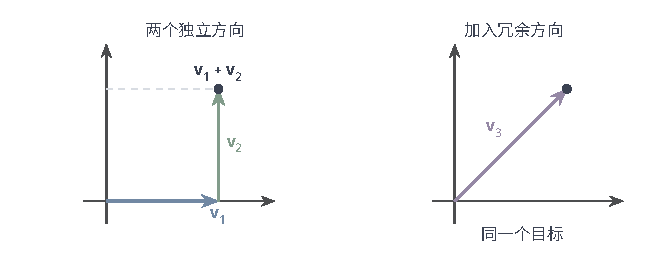
\includegraphics[width=112mm]{figures/00-shared/mathematical-preliminaries-upper/02-linear-spaces/tikz/comprehension-additions/linear-redundant-directions.pdf}
  \caption{冗余方向与重复表示。取$\bm v_1=(1,0)^{\top}$、$\bm v_2=(0,1)^{\top}$与$\bm v_3=(1,1)^{\top}$。左图沿$\bm v_1$再沿$\bm v_2$，右图直接沿$\bm v_3$，到达同一个目标；前两向量已能表示平面中的每个向量，加入$\bm v_3$只使生成组冗余。两图坐标等比例。}
  \label{fig:vol1-add-linear-redundant-directions}
\end{figure}

这个例子中的现象是一般的。存在性来自张成：张成空间之内的对象必有一组系数。唯一性来自线性无关：若同一对象有两组系数，二者相减得到式\eqref{eq:linear-algebra-independence-relation}形式的关系，无关性迫使两组系数之差为零，即两组系数完全相同。

反过来，唯一性也蕴含无关性。若存在一组不全为零的系数使线性组合为零，把这组系数加到某个对象的一组表示上，就得到同一对象的第二组表示，表示不再唯一。所以“张成空间内每个对象的系数唯一”与“零向量只有平凡表示”是同一件事的两面，这正是后面定义坐标的根据。

\subsection{基与维数}
\label{sec:ls-basis-dimension}

张成保证表示存在，无关保证表示唯一。同时满足张成和线性无关的一组向量称为\term{基}（basis）：它足够到达整个空间，又不重复，可以充当整个空间的一把“尺子”。

$\mathbb R^d$的标准坐标向量$\bm e_1,\ldots,\bm e_d$是一组基，称为标准基：$\bm x=\sum_jx_j\bm e_j$说明它们张成$\mathbb R^d$，而$\sum_ja_j\bm e_j=(a_1,\ldots,a_d)^\top=\bm0$迫使全部$a_j=0$。$P_k$中$1,t,\ldots,t^k$是一组基：每个多项式都是它们的组合，而组合为零多项式时各项系数都为零。

子空间也有基。下面为一个齐次方程的解集合求出一组基。
\begin{example}[齐次方程解平面的一组基]
\label{ex:ls-solution-plane-basis}
给定：$\mathbb R^3$中齐次方程$x_1+2x_2+3x_3=0$的解集合$N$；由示例~\ref{ex:ls-subspace-checks}，$N$是子空间。

计算：解满足$x_1=-2x_2-3x_3$，其中$x_2,x_3$可以任取，于是
\[
 \bm x=x_2(-2,1,0)^\top+x_3(-3,0,1)^\top .
\]
所以$\bm n_1=(-2,1,0)^\top$与$\bm n_2=(-3,0,1)^\top$张成$N$。若$a\bm n_1+b\bm n_2=(-2a-3b,\ a,\ b)^\top=\bm0$，比较第二、三个坐标得$a=b=0$，所以二者线性无关。

结论：$\bm n_1,\bm n_2$是$N$的一组基。
\end{example}

\paragraph{基的抽取与扩充}
若$V$有一个有限的生成组，就称$V$是有限维的；本章只讨论有限维空间。有限维空间总有基，而且可以从两个方向得到。

第一条路线是抽取。从任一有限生成组出发，若某个成员能写成其余向量的线性组合，删去它不会缩小张成范围。反复检查并删除，直到剩下的向量中没有一个能由其余向量表示。这时剩下的向量线性无关，又仍张成$V$，即构成一组基。

第二条路线是扩充。从任一线性无关组出发，逐次加入不在其张成空间中的向量。每加入一个新方向，张成范围严格扩大，新组仍线性无关：若新组的某个组合为零，新向量的系数必为零，否则新向量就能由原组表示，落在原张成空间中；新向量的系数为零以后，原组的无关性又使其余系数为零。下一小节的交换引理说明，有限维空间中线性无关组的长度不超过生成组的长度，所以扩充必在有限步内停止。停止时再也找不到张成空间之外的向量，留下的就是基。

两条路线互补：抽取把冗余的生成组压成基，扩充把线性无关组补成基。

\paragraph{维数}
\label{sec:ls-dimension}

基的向量个数是空间大小的自然度量。但先要回答一个问题：换一组基，个数会不会变？答案由交换引理给出。
\begin{theorem}[交换引理]
\label{thm:ls-exchange-lemma}
若$\bm u_1,\ldots,\bm u_r$线性无关，且每个$\bm u_i$都属于$\operatorname{span}\{\bm v_1,\ldots,\bm v_s\}$，则$r\leq s$；并且这$r$个$\bm u_i$可以逐个换入原生成组、换出同样多个$\bm v_j$，每次换完新组仍张成原来的空间。
\end{theorem}
\begin{proof}
从生成组$G_0=\{\bm v_1,\ldots,\bm v_s\}$开始。因为$\bm u_1\in\operatorname{span}G_0$，它可写成若干$\bm v_j$的组合；这些系数不能全为零，否则$\bm u_1=\bm0$，与$\bm u_1,\ldots,\bm u_r$线性无关矛盾。取某个系数非零的$\bm v_j$，从这个表达式中把它解出来，$\bm v_j$就可由$\bm u_1$与其余$\bm v$的组合表示。于是用$\bm u_1$换出$\bm v_j$，新组$G_1$与$G_0$张成同一个空间。

一般地，设第$i-1$步后的组$G_{i-1}$由$\bm u_1,\ldots,\bm u_{i-1}$和$s-(i-1)$个幸存的$\bm v$组成，且与$G_0$张成同一空间。于是$\bm u_i\in\operatorname{span}G_{i-1}$。若$\bm u_i$只用$\bm u_1,\ldots,\bm u_{i-1}$就能表示，它与前面$i-1$个方向重复，违反线性无关；所以表达式中至少一个幸存$\bm v$的系数非零，把它解出并换入$\bm u_i$，张成范围不变。只要还有幸存的$\bm v$，这一步就能做下去。

若$r>s$，换满$s$次以后组内只剩$\bm u_1,\ldots,\bm u_s$，却仍有$\bm u_{s+1}$待入列；它属于$\operatorname{span}G_s=\operatorname{span}\{\bm u_1,\ldots,\bm u_s\}$，与$r$个$\bm u$线性无关矛盾。故$r\leq s$，而上面的逐次交换正是定理要求的换入换出过程。
\end{proof}

由此，基的个数与选取无关。任取两组基，设个数分别为$r$与$s$：把第一组看成无关组、第二组看成生成组，得$r\leq s$；互换两组的角色又得$s\leq r$，所以$r=s$。这个共同的个数称为空间的\term{维数}（dimension），记为$\dim V$。只含零向量的空间以空集为基，维数为$0$。

由上一小节的例子，$\dim\mathbb R^d=d$，$\dim P_k=k+1$；方程$x_1+2x_2+3x_3=0$的解集合维数为$2$（示例~\ref{ex:ls-solution-plane-basis}），过原点的直线$\{c\bm u:c\in\mathbb R\}$（$\bm u\neq\bm0$）维数为$1$。上一节“直线”“平面”的说法现在有了确切含义。交换引理的论证依赖有限的生成组，后面的基扩充与维数计算都在这一有限维范围内进行，不能直接搬到无限维的函数展开上。

\subsection{子空间的维数与分解}
有了维数，子空间之间可以比较大小。若$U\subseteq W$，取$U$的一组基，它在$W$中仍线性无关，可以按上一小节的扩充补成$W$的基。扩充只增加向量、不删去向量，因此$\dim U\leq\dim W$；新增方向的个数恰为$\dim W-\dim U$，记录$U$之外还有多少自由度。

包含且同维时，结论收紧为相等：$\dim U=\dim W$时，把$U$的基扩充成$W$的基不需要新增任何方向，它本身已经张成$W$，故$U=W$。这里的包含条件不能省略，同维本身推不出包含。
\begin{example}[反例：同维而互不包含的两条直线]
\label{ex:ls-equal-dimension-not-nested}
给定：$\mathbb R^2$中的$U=\{(s,0)^\top:s\in\mathbb R\}$与$W=\{(s,s)^\top:s\in\mathbb R\}$。

验证：$U$以$\bm e_1$为基，$W$以$(1,1)^\top$为基，所以$\dim U=\dim W=1$。但$\bm e_1\in U$的两个坐标不相等，不在$W$中；$(1,1)^\top\in W$的第二坐标不为零，也不在$U$中。

结论：两条直线维数相同，却互不包含。维数只数方向的个数，不管这些方向具体指向哪里。
\end{example}
后面的维数公式与秩零度定理，都复用这一“先取已有基、再补新方向”的做法。

\paragraph{和的维数公式}
和空间的维数不是两边维数的简单相加，因为公共方向会被重复计入。

设$\bm z_1,\ldots,\bm z_k$是$U\cap W$的一组基，把它扩充为$U$的基$\bm z_1,\ldots,\bm z_k,\bm u_1,\ldots,\bm u_p$，再另行扩充为$W$的基$\bm z_1,\ldots,\bm z_k,\bm w_1,\ldots,\bm w_q$。下面说明这$k+p+q$个向量构成$U+W$的基。

它们张成$U+W$，因为每个$\bm u+\bm w$（$\bm u\in U$，$\bm w\in W$）都是两组基的组合。为证线性无关，设
\[
 \sum_i\alpha_i\bm z_i+\sum_j\beta_j\bm u_j+\sum_l\gamma_l\bm w_l=\bm0 .
\]
移项得$\sum_l\gamma_l\bm w_l=-\sum_i\alpha_i\bm z_i-\sum_j\beta_j\bm u_j$。左边属于$W$，右边属于$U$，所以这个向量属于$U\cap W$，可以写成$\sum_i\delta_i\bm z_i$。于是$\sum_l\gamma_l\bm w_l-\sum_i\delta_i\bm z_i=\bm0$，由$W$的基线性无关，全部$\gamma_l=0$。代回原式，再由$U$的基线性无关，全部$\alpha_i$与$\beta_j$也为零。因此$\dim(U+W)=k+p+q=(k+p)+(k+q)-k$，即
\begin{equation}
 \dim(U+W)=\dim U+\dim W-\dim(U\cap W).
 \label{eq:ls-dimension-formula}
\end{equation}
被减去的维数正是两边重复计入的公共方向，而不是两个集合元素个数的差。下面在$\mathbb R^3$中核对这一公式。
\begin{example}[两个坐标平面的和]
\label{ex:ls-dimension-formula-planes}
给定：$\mathbb R^3$中的$U=\operatorname{span}\{\bm e_1,\bm e_2\}$与$W=\operatorname{span}\{\bm e_2,\bm e_3\}$。

计算：$U$由第三坐标为零的向量组成，$W$由第一坐标为零的向量组成，所以$U\cap W$由第一、三坐标都为零的向量组成，即$U\cap W=\operatorname{span}\{\bm e_2\}$，维数为$1$。$U+W$含有$\bm e_1,\bm e_2,\bm e_3$，所以$U+W=\mathbb R^3$。代入公式：
\[
 \dim(U+W)=3=2+2-1 .
\]
若改取两条坐标轴$U'=\operatorname{span}\{\bm e_1\}$、$W'=\operatorname{span}\{\bm e_2\}$，交为零，$\dim(U'+W')=1+1-0=2$。

结论：公式中减去的$1$正是两个平面共有的$\bm e_2$方向；交为零时，和的维数等于两边维数之和。
\end{example}

\paragraph{补空间的存在}
第~\ref{sec:ls-direct-sum}节定义了补空间，现在可以说明它总存在。把$U$的基扩充为$V$的基，新增向量张成的子空间记为$W$。整组基张成$V$，所以$U+W=V$。若某向量同属$U$与$W$，它既是$U$的基向量的组合，又是新增向量的组合，两种写法相减，得到整组基的一个组合为零，系数只能全为零，所以$U\cap W=\{\bm0\}$。于是$V=U\oplus W$。由维数公式，直和时交的维数为零，$\dim V=\dim U+\dim W$。扩充的选择不唯一，补空间也就不唯一，这与平面中直线的例子一致。

\paragraph{商空间的维数}
同样的“先取已有基、再补新方向”也回答了第~\ref{sec:ls-quotient-spaces}节留下的问题：商空间$V/U$有多少个独立方向？取$U$的一组基$\bm u_1,\ldots,\bm u_s$并扩充为$V$的基$\bm u_1,\ldots,\bm u_s,\bm w_1,\ldots,\bm w_t$。新增向量的类$\bm w_1+U,\ldots,\bm w_t+U$张成$V/U$：任一$\bm x$写成整组基的组合，其中$U$部分落进零类被消去。

这些类也线性无关：若$\sum_ja_j(\bm w_j+U)=U$，则$\sum_ja_j\bm w_j\in U$，它能由$\bm u_i$表示，整组基的线性无关性迫使全部$a_j=0$。因此
\begin{equation}
 \dim(V/U)=\dim V-\dim U.
 \label{eq:ls-quotient-dimension}
\end{equation}

商空间的维数恰好等于补空间的维数。新增方向$\bm w_j$张成$U$的一个补空间$W$，每个$\bm x$唯一分解为$\bm x=\bm u+\bm w$（$\bm u\in U$，$\bm w\in W$），于是类$\bm x+U=\bm w+U$中的点都形如$\bm w+\bm u'$（$\bm u'\in U$）。这样的点落在$W$中当且仅当$\bm u'\in U\cap W=\{\bm0\}$，所以每个类与$W$恰交于一点$\bm w$。选定补空间，就是为每个类选定一个代表元。补空间要选，商空间却不依赖任何选择，这是二者的区别。

示例~\ref{ex:ls-quotient-intercept}中，$\dim(P_1/U)=2-1=1$，商空间只剩截距这一个方向；图~\ref{fig:ls-quotient-equivalence-classes}中，$\dim(\mathbb R^2/U)=1$，只剩高度。

\subsection{坐标与坐标变换}
\label{sec:ls-coordinates}
\label{sec:linear-algebra-coordinates}

有了基，每个对象都有唯一的一组系数。怎样用这组系数代替对象参与计算？代替以后，系数的大小能否反映对象的大小？换一组基，系数怎样换算？本小节依次回答这三个问题。

\paragraph{有序基下的坐标}
固定有序基$\mathcal B=(\bm b_1,\ldots,\bm b_d)$后，对象$\bm v$唯一写成$\sum_{j=1}^d x_j\bm b_j$。系数列$[\bm v]_{\mathcal B}=(x_1,\ldots,x_d)^{\top}$称为$\bm v$在基$\mathcal B$下的\term{坐标}（coordinates）。

存在性来自张成，唯一性来自线性无关，所以坐标映射$\bm v\mapsto[\bm v]_{\mathcal B}$是从$V$到$\mathbb R^d$的双射：每个对象恰有一列坐标，每列实数$(x_1,\ldots,x_d)^{\top}$也恰好记录对象$\sum_jx_j\bm b_j$。

它还保持线性组合：若$[\bm v]_{\mathcal B}=\bm x$、$[\bm w]_{\mathcal B}=\bm y$，则$a\bm v+b\bm w=\sum_j(ax_j+by_j)\bm b_j$，由唯一性得$[a\bm v+b\bm w]_{\mathcal B}=a\bm x+b\bm y$。因此对象上的线性运算可以完全交给坐标去算，算完再按基还原。

在$\mathbb R^d$中，把基向量排成矩阵$\bm B=[\bm b_1\ \cdots\ \bm b_d]$，按列读法$\bm v=\bm B[\bm v]_{\mathcal B}$，所以坐标就是方程$\bm B\bm x=\bm v$的唯一解。下面用这一方程求一个斜基下的坐标。
\begin{example}[同一向量在两组基下的坐标]
\label{ex:ls-coordinates-two-bases}
给定：$\mathbb R^2$中的向量$\bm x=(1,2)^\top$，标准基$(\bm e_1,\bm e_2)$，以及斜基$\mathcal B=(\bm b_1,\bm b_2)$，$\bm b_1=(2,1)^\top$、$\bm b_2=(-1,1)^\top$。

计算：标准基下$\bm x=1\cdot\bm e_1+2\cdot\bm e_2$，坐标为$(1,2)^\top$。斜基下的坐标$(c_1,c_2)^\top$满足$c_1\bm b_1+c_2\bm b_2=\bm x$，即
\[
 \begin{gathered}
2c_1-c_2=1\\
c_1+c_2=2 .
 \end{gathered}
\]
两式相加得$3c_1=3$，所以$c_1=1$、$c_2=1$。核对：$\bm b_1+\bm b_2=(1,2)^\top$。

结论：$[\bm x]_{\mathcal B}=(1,1)^\top$。向量本身没有移动，只是沿不同的基去量。
\end{example}
图~\ref{fig:ls-basis-coordinates}画出这两种读法。
\begin{figure*}[htbp]
  \centering
  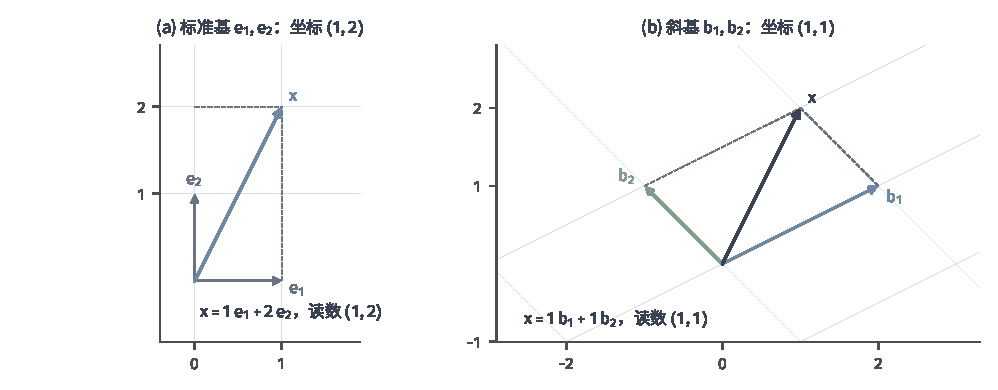
\includegraphics[width=169mm]{figures/00-shared/mathematical-preliminaries-upper/02-linear-spaces/matplotlib/ls-basis-coordinates/ls-basis-coordinates.pdf}
  \caption{同一向量在两组基下的坐标。左：标准基$\bm e_1,\bm e_2$（灰箭头）下，向量$\bm x=(1,2)$（蓝箭头）的坐标为$(1,2)$，虚线为向坐标轴的垂线。右：斜基$\bm b_1=(2,1)$（蓝）、$\bm b_2=(-1,1)$（绿）下，同一个$\bm x$满足$\bm x=\bm b_1+\bm b_2$，坐标为$(1,1)$，浅色斜线为斜基网格，虚线为平行四边形读法。两图坐标系相同。}
  \label{fig:ls-basis-coordinates}
\end{figure*}

\paragraph{坐标与对象}
坐标列要与它所记录的对象区分开：几何位移、有限信号、多项式都可以相加和缩放，它们是\emph{对象}；一列实数只是选定基以后记录对象的\emph{坐标}。基的顺序也要固定：交换$\bm b_1,\bm b_2$，对象不变，坐标列的前两个数也随之交换。在$\mathbb R^d$中直接写数字列，通常是默认使用标准基$\bm e_1,\ldots,\bm e_d$，这时对象与坐标恰好是同一列数，第~\ref{chap:linear-operations}章正是在这种默认下工作的。

函数的基展开则必须区分二者：函数是对象，展开系数是坐标。
\begin{example}[仿射函数在两组基下的坐标]
\label{ex:ls-affine-function-coordinates}
给定：$P_1$中的$f_{a,b}=a+bt$，以及两组基$\mathcal B_1=(1,t)$与$\mathcal B_2=(1,1+t)$。

计算：在$\mathcal B_1$下$f_{a,b}=a\cdot1+b\cdot t$，坐标为$(a,b)^\top$。在$\mathcal B_2$下设$f_{a,b}=c_1\cdot1+c_2(1+t)=(c_1+c_2)+c_2t$，比较常数项与$t$的系数，得$c_2=b$、$c_1=a-b$，即
\[
 f_{a,b}=(a-b)\cdot1+b\cdot(1+t).
\]

结论：同一个函数在$\mathcal B_1$与$\mathcal B_2$下的坐标分别是$(a,b)^\top$与$(a-b,b)^\top$；坐标改变了，函数本身没有改变。
\end{example}
坐标的个数总是维数。一个对象若用冗余的生成组记录，记录的长度可以超过维数，所以不能由这种记录的长度推断空间有几维。

\paragraph{坐标对基的敏感性}
对象不变时，坐标仍可能相差很大。贯穿例给出一个数值上很极端的情形。
\begin{example}[近共线基下的大坐标]
\label{ex:ls-coordinate-instability}
给定：示例~\ref{ex:ls-nearly-collinear-independence}中的$\bm c_1,\bm q$与$\bm c_2=\bm c_1+\varepsilon\bm q$（$\varepsilon\neq0$），$\delta=0.1$，以及目标向量
\begin{equation}
 \bm y=\bm c_1+\delta\bm q=\begin{bmatrix}1\\1.1\\0.9\end{bmatrix}.
 \label{eq:linear-algebra-nearly-collinear-target}
\end{equation}
由该示例，$\mathcal B_0=(\bm c_1,\bm q)$与$\mathcal B_\varepsilon=(\bm c_1,\bm c_2)$都是平面$\operatorname{span}\{\bm c_1,\bm q\}$的基，$\bm y$也在这个平面中。

计算：在$\mathcal B_0$下，$\bm y$的坐标是$(1,\delta)^{\top}$。在$\mathcal B_\varepsilon$下，把$\bm q=(\bm c_2-\bm c_1)/\varepsilon$代入$\bm y=\bm c_1+\delta\bm q$，得
\begin{equation}
 \bm y=\left(1-\frac{\delta}{\varepsilon}\right)\bm c_1
       +\frac{\delta}{\varepsilon}\bm c_2.
 \label{eq:linear-algebra-coordinate-instability}
\end{equation}
取$\varepsilon=0.01$，则$\delta/\varepsilon=10$，坐标成为$(-9,10)^{\top}$。

结论：同一个$\bm y$在$\mathcal B_0$下的坐标为$(1,0.1)^\top$，在$\mathcal B_{0.01}$下的坐标为$(-9,10)^\top$。
\end{example}
两个很大的系数在几乎同向的两个基向量上相互抵消，不能据此判断原对象很大。这种系数对接近退化的基的敏感，将在第~\ref{chap:linear-analysis}章定量讨论。新旧坐标之间怎样系统地换算，是下面要回答的问题。

\paragraph{换基矩阵}
\phantomsection
\label{sec:ls-change-basis}
\label{sec:linear-algebra-coordinate-conversions}
设$\mathcal B=(\bm b_1,\ldots,\bm b_d)$与$\mathcal C$是$V$的两组有序基。已知$\bm v$在$\mathcal B$下的坐标$[\bm v]_{\mathcal B}=(x_1,\ldots,x_d)^{\top}$，怎样求它在$\mathcal C$下的坐标？由$\bm v=\sum_jx_j\bm b_j$，并且坐标映射保持线性组合，
\[
 [\bm v]_{\mathcal C}=\sum_{j=1}^d x_j[\bm b_j]_{\mathcal C}.
\]
右边是各列$[\bm b_j]_{\mathcal C}$以$x_j$为权重的线性组合。把这些列排成矩阵，称为从$\mathcal B$到$\mathcal C$的换基矩阵$\bm S_{\mathcal C\leftarrow\mathcal B}$，按矩阵与向量乘积的列读法，
\begin{equation}
 [\bm v]_{\mathcal C}
 =\bm S_{\mathcal C\leftarrow\mathcal B}[\bm v]_{\mathcal B}.
 \label{eq:linear-algebra-coordinate-change}
\end{equation}
换基矩阵的第$j$列是旧基向量$\bm b_j$的新坐标；下标$\mathcal C\leftarrow\mathcal B$从右向左读，表示把$\mathcal B$坐标译成$\mathcal C$坐标。下面在平面上算一个具体的换基矩阵。
\begin{example}[平面上的换基矩阵]
\label{ex:ls-change-of-basis-plane}
给定：$\mathbb R^2$的标准基$\mathcal E$与基$\mathcal U=(\bm u_1,\bm u_2)$，$\bm u_1=(1,0)^{\top}$、$\bm u_2=(1,1)^{\top}$；向量$\bm v$在$\mathcal U$下的坐标为$(1,1)^\top$。

计算：$\bm u_1,\bm u_2$的标准坐标就是它们自己。按“第$j$列是旧基向量的新坐标”，
\[
 \bm S_{\mathcal E\leftarrow\mathcal U}=\begin{bmatrix}1&1\\0&1\end{bmatrix}.
\]
由式~\eqref{eq:linear-algebra-coordinate-change}，$[\bm v]_{\mathcal E}=\bm S_{\mathcal E\leftarrow\mathcal U}(1,1)^{\top}=(2,1)^{\top}$。直接核对：$\bm v=\bm u_1+\bm u_2=(2,1)^\top$。

结论：$\mathcal U$坐标$(1,1)^\top$与标准坐标$(2,1)^\top$记录的是同一个向量。
\end{example}
图~\ref{fig:vol1-add-linear-change-basis}画出这一点：目标位置没有移动，改变的只是沿哪两条基方向累加，以及每条方向取多少份。
\begin{figure}[!htb]
  \centering
  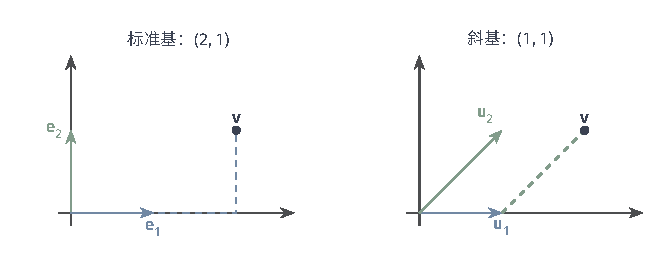
\includegraphics[width=112mm]{figures/00-shared/mathematical-preliminaries-upper/02-linear-spaces/tikz/comprehension-additions/linear-change-basis.pdf}
  \caption{同一向量的两套坐标。左图使用标准基，$\bm v=(2,1)^{\top}$的坐标为$(2,1)^{\top}$；右图使用$\bm u_1=(1,0)^{\top}$、$\bm u_2=(1,1)^{\top}$，同一$\bm v$的坐标为$(1,1)^{\top}$。虚线表示相应的向量相加，两图的环境坐标比例相同。}
  \label{fig:vol1-add-linear-change-basis}
\end{figure}

\paragraph{连续换基与反向换基}
若再换到第三组基$\mathcal D$，中间那套坐标应当不留痕迹。对每个$\bm v$，连用两次式~\eqref{eq:linear-algebra-coordinate-change}，
\[
 [\bm v]_{\mathcal D}=\bm S_{\mathcal D\leftarrow\mathcal C}[\bm v]_{\mathcal C}=\bm S_{\mathcal D\leftarrow\mathcal C}\bm S_{\mathcal C\leftarrow\mathcal B}[\bm v]_{\mathcal B}.
\]
取$\bm v=\bm b_j$，它的$\mathcal B$坐标是$\bm e_j$，两边读出的分别是$\bm S_{\mathcal D\leftarrow\mathcal B}$与乘积的第$j$列，所以
\[
 \bm S_{\mathcal D\leftarrow\mathcal B}
 =\bm S_{\mathcal D\leftarrow\mathcal C}\bm S_{\mathcal C\leftarrow\mathcal B}.
\]

特别取$\mathcal D=\mathcal B$。每个$\bm b_j$在$\mathcal B$下的坐标是$\bm e_j$，所以左边$\bm S_{\mathcal B\leftarrow\mathcal B}=\bm I_d$，即$\bm S_{\mathcal B\leftarrow\mathcal C}\bm S_{\mathcal C\leftarrow\mathcal B}=\bm I_d$；交换两组基的角色，同理得$\bm S_{\mathcal C\leftarrow\mathcal B}\bm S_{\mathcal B\leftarrow\mathcal C}=\bm I_d$。所以换基矩阵总可逆，反向换基矩阵就是它的逆：$\bm S_{\mathcal B\leftarrow\mathcal C}=\bm S_{\mathcal C\leftarrow\mathcal B}^{-1}$。在示例~\ref{ex:ls-change-of-basis-plane}中，$\bm S_{\mathcal U\leftarrow\mathcal E}=\bm S_{\mathcal E\leftarrow\mathcal U}^{-1}=\left[\begin{smallmatrix}1&-1\\0&1\end{smallmatrix}\right]$，它把$(2,1)^{\top}$送回$(1,1)^{\top}$。

反过来，任一$d$阶可逆矩阵$\bm P$都是某次换基的矩阵。以$\bm P$的第$j$列为$\mathcal B$坐标，取向量$\bm b'_j=\sum_i\bm P_{i,j}\bm b_i$。$\bm P$的列线性无关，而坐标映射是保持线性组合的双射，所以$\bm b'_1,\ldots,\bm b'_d$也线性无关。个数等于维数的线性无关组必是基：否则它还能扩充，得到多于$\dim V$个线性无关的向量，与交换引理矛盾。于是$\bm b'_1,\ldots,\bm b'_d$构成一组基$\mathcal B'$。按定义，$\bm S_{\mathcal B\leftarrow\mathcal B'}$的第$j$列是$\bm b'_j$的$\mathcal B$坐标，即$\bm P$的第$j$列，所以$\bm S_{\mathcal B\leftarrow\mathcal B'}=\bm P$。

反向换基的代价取决于换基矩阵是否接近不可逆。贯穿例把这一点表现得很清楚。
\begin{example}[近共线基之间的换基]
\label{ex:ls-nearly-collinear-change-of-basis}
给定：示例~\ref{ex:ls-coordinate-instability}中的两组基$\mathcal B_0=(\bm c_1,\bm q)$与$\mathcal B_\varepsilon=(\bm c_1,\bm c_2)$，$\varepsilon\neq0$。

计算：由$\bm c_1=1\cdot\bm c_1+0\cdot\bm q$与$\bm c_2=1\cdot\bm c_1+\varepsilon\bm q$，$\mathcal B_\varepsilon$的两个向量在$\mathcal B_0$下的坐标分别是$(1,0)^{\top}$与$(1,\varepsilon)^{\top}$，所以
\[
\begin{gathered}
\bm S_{\mathcal B_0\leftarrow\mathcal B_\varepsilon}
 =\begin{bmatrix}1&1\\0&\varepsilon\end{bmatrix}\\
\bm S_{\mathcal B_\varepsilon\leftarrow\mathcal B_0}
 =\bm S_{\mathcal B_0\leftarrow\mathcal B_\varepsilon}^{-1}
 =\begin{bmatrix}1&-1/\varepsilon\\0&1/\varepsilon\end{bmatrix},
\end{gathered}
\]
后者可由直接相乘验证。把$\bm y$在$\mathcal B_0$下的坐标$(1,\delta)^{\top}$代入后者，得
\[
 \bm S_{\mathcal B_\varepsilon\leftarrow\mathcal B_0}\begin{bmatrix}1\\\delta\end{bmatrix}
 =\begin{bmatrix}1-\delta/\varepsilon\\\delta/\varepsilon\end{bmatrix},
\]
与式~\eqref{eq:linear-algebra-coordinate-instability}一致。

结论：$\bm S_{\mathcal B_0\leftarrow\mathcal B_\varepsilon}$的行列式为$\varepsilon$，接近零；反向换基矩阵含有因子$1/\varepsilon$，小的基差异由此被放大成大系数。
\end{example}

\paragraph{被动换基与主动作用}
被动换基与主动作用必须分开。换基时对象不动、记录改变，式\eqref{eq:linear-algebra-coordinate-change}两侧是同一个$\bm v$的两套坐标；主动作用则在固定的坐标下把对象送到另一个对象，例如第~\ref{chap:linear-operations}章的矩阵作用$\bm x\mapsto\bm A\bm x$把向量旋转或切变，下一节把它推广为线性映射。

两者都写成矩阵乘以坐标列，形式相似，含义不同。下面的例子在同一个初始向量上比较两种情形。
\begin{example}[被动换基与主动切变]
\label{ex:ls-passive-vs-active}
给定：$\mathbb R^2$中的向量$\bm x=(3,3)^\top$，斜基$\mathcal B'=(\bm b_1,\bm b_2)$，$\bm b_1=(2,1)^\top$、$\bm b_2=(-1,1)^\top$，以及切变矩阵$\bm A=\left[\begin{smallmatrix}1&1\\0&1\end{smallmatrix}\right]$。

计算：被动换基时，求$\bm x$在$\mathcal B'$下的坐标$(c_1,c_2)^\top$。由$2c_1-c_2=3$与$c_1+c_2=3$得$c_1=2$、$c_2=1$，即$\bm x=2\bm b_1+\bm b_2$。主动作用时，计算$\bm A\bm x=(3+3,\ 3)^\top=(6,3)^\top$。

结论：前者中向量仍是$(3,3)^\top$，只是读数从$(3,3)$变成$(2,1)$；后者中坐标系不动，向量本身被搬到$(6,3)^\top$。
\end{example}
图~\ref{fig:ls-passive-change-vs-active-map}把两种情形并排画出。所以不能把所有乘矩阵的运算都理解成换基。
\begin{figure*}[htbp]
  \centering
  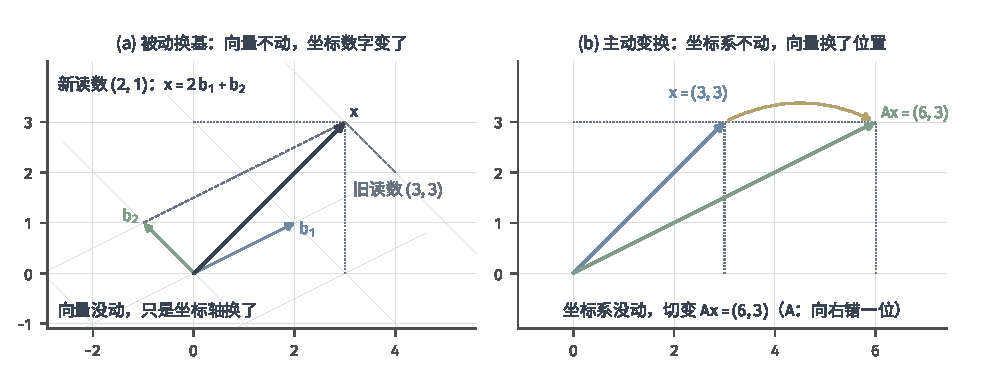
\includegraphics[width=169mm]{figures/00-shared/mathematical-preliminaries-upper/02-linear-spaces/matplotlib/ls-passive-change-vs-active-map/ls-passive-change-vs-active-map.pdf}
  \caption{被动换基与主动变换的对照，两图使用同一个初始向量$\bm x=(3,3)$。左（被动换基）：箭头位置不动（深色），旧标准读数用点线投影读出$(3,3)$；新斜基$\bm b_1=(2,1)$（蓝）、$\bm b_2=(-1,1)$（绿）与浅色斜网格下，$\bm x=2\bm b_1+\bm b_2$，新读数为$(2,1)$。右（主动变换）：标准坐标系不动，$\bm x$（蓝）被切变映到$\bm A\bm x=(6,3)$（绿），黄色弧线表示搬动过程。}
  \label{fig:ls-passive-change-vs-active-map}
\end{figure*}
